% this package changes the paragraph style to skip a line before a new paragraph rather than indenting% font size
\documentclass[11pt]{article}
\usepackage{fullpage,parskip,amsmath,amssymb,algorithm2e,enumitem,graphicx}
\usepackage{hyperref}
\usepackage{graphicx}
\usepackage{wrapfig}

\hypersetup{
    colorlinks=true,
    linkcolor=blue,
    filecolor=magenta,      
    urlcolor=blue,
    pdftitle={Overleaf Example},
    pdfpagemode=FullScreen,
    }
\usepackage{xcolor}

\parindent24pt
\pagestyle{empty}

\newcommand{\n}{\newcommand%
}
\renewcommand{\r}{\renewcommand%
}
\SetAlgoLined
\r{\bf}{\textbf}
\r{\it}{\textit}
\n{\ol}{\overline}
\n{\ul}{\underline}
\n{\unspace}{\vspace{-2.15em}}
\AtBeginEnvironment{align}{\setcounter{equation}{0}\vspace{-18pt}}
\AtBeginEnvironment{flalign}{\setcounter{equation}{0}}
\AtBeginEnvironment{align}{\unspace}
\AtBeginEnvironment{align*}{\unspace}
\AtBeginEnvironment{flalign}{\unspace}
\AtBeginEnvironment{flalign*}{\unspace}
\AtBeginEnvironment{algorithm}{\Indp}
\setenumerate[1]{label=\bf{(\arabic*)}}
\n{\note}[1]{\it{Note: }#1}
\newenvironment{proof}[1]{\it{pf: }This is a proof by #1.\par \begin{itemize}}{\end{itemize}}
\SetKwBlock{Blk}{}{}
\n{\Fn}[3]{\KwSty{Function} \ArgSty{#1(#2)}\Blk{#3}}


\begin{document}

\noindent\boxed{
\begin{tabular*}{\textwidth}{@{}l@{\extracolsep{\fill}}r@{}}
CSCI 2600 --- Principles of Software\\\\
\multicolumn{2}{c}{\huge{Homework 4: Designing and Implementing an ADT}}\\
\multicolumn{2}{c}{\it{Due: Monday, March 27, 2023,  11:59:59 pm}}\\\\
\end{tabular*}}
\par
\noindent We recommend that you read the \textbf{entire} homework before you begin work. As always, you must commit and push to your Git repository, then submit on \href{https://submitty.cs.rpi.edu/courses/s23/csci2600}{Submitty}.
\newline

\noindent {\huge\textbf{\underline{Submission Instructions}}}
\begin{itemize}
\item  
Follow the directions in the \href{https://www.cs.rpi.edu/academics/courses/spring23/csci2600/Documents/eclipse_and_git.pdf}{version control handout} for cloning your hw04 git repo. The URI that you will need to use to clone your personal repo for this homework would have the form of \texttt{https://submitty.cs.rpi.edu/git/s23/csci2600/hw04/RCSID} where RCSID is your RCS ID.

\item
Be sure to commit and push the files to Submitty. Follow the directions in the \href{https://www.cs.rpi.edu/academics/courses/spring23/csci2600/Documents/eclipse_and_git.pdf}{version control handout} for adding and committing files.

\item
Be sure to add any additional files to your repo using Team/Add to Index.

\item
\textcolor{red}{\textbf{Important:} You must press the \textbf{Grade My Repository} button, or your answers will not be graded.}
\end{itemize}

\noindent {\huge\textbf{\underline{Introduction}}}
\newline

\noindent In this assignment, you will design, implement, and test a graph ADT. Given an abstract, high-level description of the desired ADT, you will develop a working Java implementation. You get to choose both the public interface and internal representation, then decide what unit tests to write to demonstrate that your implementation works correctly.
\newline

\noindent This assignment is the first part of a multi-part project. In subsequent assignments you will build several clients of your graph ADT.
\newpage
\noindent {\huge\textbf{\underline{Building a Graph}}}
\newline
\section*{Definitions and Terminology:}
\label{sec:Definitions and Terminology}

A graph is a collection of nodes (also called vertices) and edges (also called links). Each edge connects two nodes. In a directed graph, edges are one-way: an edge e = ⟨A,B⟩ indicates B that is directly reachable from A. To indicate that B is directly reachable from A and A from B, a directed graph would have edges ⟨A,B⟩ and ⟨B,A⟩.


\noindent The children of node B are the nodes to which there is an edge from B. In Fig. 1, the children of b are a and c. Similarly, the parents of B are the nodes from which there is an edge to B. In Fig. 1, b only has one parent, a.

\noindent A path is a sequence of edges ⟨node1,node2⟩, ⟨node2,node3⟩, ⟨node3,node4⟩, .... In other words, a path is an ordered list of edges, where an edge to some node is immediately followed by an edge from that node. In Fig. 1, one possible path is ⟨b,a⟩,⟨a,b⟩,⟨b,c⟩. This path represents traveling from b to a to b to c. A path may traverse a given edge more than once.

\noindent A reflexive edge is an edge which starts and ends at the same node. In Fig 1. there is a reflexive edge from a to a: ⟨a,a⟩. Your graph implementation must allow for reflexive edges.
\newline
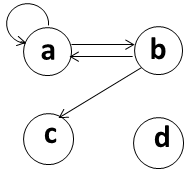
\includegraphics[]{digraph.png}
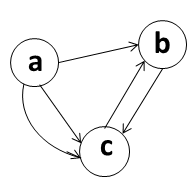
\includegraphics[]{multigraph.png}
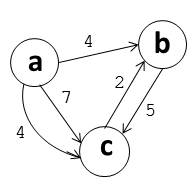
\includegraphics[]{labeled-graph.png}
\newline
Figure 1: A simple directed \hspace{4em} Figure 2: A directed \hspace{2em} Figure 3:  A directed labeled
\newline
graph with four nodes. \hspace{6em}multigraph. \hspace{6em}multigraph.
\newpage
\noindent In a multigraph, there can be any number of edges (zero, one, or more) between a pair of nodes. Fig. 2 shows a multigraph with 2 edges from a to c.

\noindent In a labeled graph (Fig. 3), every edge has a label containing information of some sort. Labels are not unique: multiple edges may have the same label. In theory, a graph could contain two "identical" edges with the same starting point, ending point, and label, but for this project you may decide whether to allow identical edges in your implementation. (Whatever you decide, make sure it is clearly documented so clients understand how they can use your ADT.)

\noindent If you want to learn more, read \href{http://en.wikipedia.org/wiki/Graph_%28data_structure%29}{Wikipedia's definition of a graph.} Then if you still have a question, ask us.

\noindent Many interesting problems can be represented with graphs. For example:
\begin{itemize}

\item A graph can represent airline flights between cities, where each city is a node and an edge ⟨A,B⟩ indicates that there is a flight from A to B. The edge label might represent the cost in money (airfare), time (length of flight), or distance.
\item To find walking routes across RPI's campus in Troy, you can build a graph where nodes represent buildings and other locations and edges represent walking paths connecting two locations. The label/cost of an edge is the physical length of that path.
\item The Web can be modeled as a graph with node for every Webpage and an edge ⟨A,B⟩ if page A links to page B. The label could indicate the anchor text for a link on page A, or the number of links from page A to page B.
\item Facebook is essentially a giant graph with nodes for users and edges between friends. (You can see a \href{https://engineering.fb.com/2010/12/13/core-data/visualizing-friendships/}{visualization of the Facebook graph.})
\end{itemize}
\newpage

\section*{Problem 1: Write a Specification for Graph}
\label{sec:Problem 1}

\noindent To start, you will specify the API for a Java class or classes representing a directed labeled multigraph. The API, or public interface, is the collection of public classes and methods that clients of your graph ADT will use. We recommend that you work in iterative layers of detail. Start rough — preferably with pencil and paper — by brainstorming what operations the ADT needs to support, how it might be logically broken into modules (classes/interfaces), and how these modules connect to each other. Then, jot down a list of methods for each class that provide these operations. Think through some possible client applications, particularly finding efficient routes between different nodes, to get an idea about what operations might be needed.

\noindent Initially you should keep your design rough — don't write formal class and method specifications with all the proper clauses right away. Your design will likely go through multiple iterations, and it's easier to throw away parts before you've invested too much effort in them.

\noindent Once you are satisfied with your high-level design, write a specification for each class and method. Follow the convention we have been using in this class, remembering to use both standard Javadoc tags (\texttt{param, returns, throws}) and the ones introduced for this course (\texttt{requires, effects, modifies, etc.}) Go over \href{https://www.cs.rpi.edu/academics/courses/spring23/csci2600/Slides/Specifications.pdf}{the slides for specifications again.} A good approach is to create skeleton implementations of your classes containing only method “stubs”, then write your specifications in place in the code. A stub is a not-yet-implemented method whose body simply throws an exception, as you saw in the Homework 3 starter code. Stubbing out a class gives you the flexibility to write client code and tests that use it before completing the implementation. The skeleton code will not behave correctly or pass tests, but the program will compile and run.

\noindent For this assignment, you may restrict your graph to store the data in nodes and edge labels as \texttt{String}s. We strongly recommend you DO NOT use generics for this assignment. In a future assignment, you will use generics to make your ADT work with other data types — text, integers, doubles, etc. You may assume nodes are uniquely identified by their data contents: that is, no two nodes store the same data.

\noindent Design problems such as this one are open-ended by nature: we are not looking for one “right” design. There are principles of good design you have learned in lecture, however. You will also find suggestions of what to consider and how to approach the problem in the \hyperref[sec:Hints]{hints} section. Also, designs naturally evolve as requirements change, so try to make your code extensible, but don't over-generalize.

\noindent Once you are done with the specification of your Graph ADT (overview, AF, and representation invariant and Principles of Software specifications for each abstract operation) copy and paste your specs and stubs into the file \texttt{answers/hw4\_problem1.pdf}. You can use \texttt{RatNum.java} from hw3 as a guide.

\newpage

\section*{Problem 2: Write Tests for Graph}
\label{sec:Problem 2}

Write a black-box test suite for your Graph specifications. It is important to write your tests before your code, but your tests will not pass until you have completed \hyperref[sec:Problem 3]{Problem 3}.

\begin{itemize}
\item \textbf{Documentation}: Include with your test cases one short paragraph of documentation explaining your testing strategy, and which (if any) testing heuristics you used. Place this write-up in \texttt{answers/hw4\_problem2.pdf}.
\end{itemize}

\noindent Create and commit new JUnit test classes in directory \texttt{src/test/java/hw4}. You must have a JUnit test case for \texttt{GraphWrapper} placed into file \texttt{src/test/java/hw4/GraphWrapperTest.java} which should already exist in your repository. (\texttt{GraphWrapper} is explained in \hyperref[sec:Problem 3]{Problem 3}.) You may need to add other files later on. To create a new test case, right-click on \texttt{hw4} under \texttt{src/test/java}, then New -$>$ JUnit Test Case, then type a name for the new test class. Don't forget to add JUnit to the build path! Look back to Homework 0 and Homework 3 as examples of extensive test suites.

\section*{Problem 3: Implement Graph}
\label{sec:Problem 3}
A Java source code file \texttt{GraphWrapper.java} for the \texttt{GraphWrapper} class (it is explained shortly after) should already exist in your repository. When you later need to add other Java source code files, right-click on \texttt{hw4} under \texttt{src/main/java}, then New -$>$ Class, Package: \texttt{hw4}, and then enter the name of the class to be created. Be sure to use \texttt{Team/Add to Index} to add the file to your repo.

\noindent There are many ways to \href{http://en.wikipedia.org/wiki/Graph_%28data_structure%29#Representations}{represent} a graph. Here are a few:
\begin{itemize}
\item As a collection of edges.
\item As an adjacency list, in which each node is associated with a list of its outgoing edges.
\item As an adjacency matrix, which explicitly represents, for every pair ⟨A,B⟩ of edges, whether there is a link from A to B, and how many.
\end{itemize}

\begin{enumerate}
\item In one brief paragraph, describe your representation. For at least the three representations above and your representation (if it is not one of the ones above), explain an advantage of that representation in a sentence. For example, do certain representations have advantages of efficiency in search or ease of implementation. Given these advantages, briefly explain why you chose the representation you did. You should place this discussion in a file called \texttt{answers/hw4\_problem3.pdf}.
\newpage

\item Place a proper \textbf{abstraction function and representation invariant} for your Graph data type (and any other ADTs you create) in your source code. Also implement a private \texttt{checkRep()} method, which will help in finding errors in your implementation. You do not need a representation invariant or abstraction function for \texttt{GraphWrapper.java}. It is not an ADT.
\item Provide an implementation of your graph data type. We ask that you strive first for a good design before worrying about performance right now. Eventually, however, your path-finding application will create and operate on very large graphs, so the scalability of your Graph implementation will be important. Since the path-finding algorithm must frequently look up the children for a given node, this operation should be performed quickly even for large graph sizes. Your graph building operations should also be reasonably efficient. As your implementation will likely use classes in the Java Collections Framework, you should understand the computational complexity of classes such as \href{https://docs.oracle.com/javase/8/docs/api/java/util/HashMap.html}{HashMap} and \href{http://docs.oracle.com/javase/8/docs/api/java/util/ArrayList.html}{ArrayList}.
\item Be sure to call your \texttt{checkRep()} where appropriate.
\item
Once you've finished your implementation, you should think about whether or not new tests are needed in addition to those you wrote before you started coding. If so, you should add these to your test suite. You should \textbf{append to the end of your test strategy writeup} in \hyperref[sec:Problem 2]{Problem 2} a description of any new tests you added, or why you feel that your original tests alone are sufficient. At this point you will use \href{http://www.eclemma.org/}{\textbf{EclEmma}} (available through the Eclipse Marketplace), which measures your code coverage. Look for coverage of package \texttt{hw4} in EclEmma. You must achieve 75\% or higher coverage for \texttt{hw4} to receive full credit on this part. We measure the coverage of your Java code as executed by your test suite.
\item
If EclEmma is not already installed in Eclipse, select \texttt{Help} from the main menu and then select \texttt{Eclipse Marketplace}. In the search box, enter \texttt{EclEmma}. Select \texttt{Install} to begin the installation.
\end{enumerate}

\noindent You have freedom to design the Graph ADT as you wish (you can name your class, include operations at your discretion, and choose the rep as you like). However, we require that you implement an additional class, \texttt{GraphWrapper}, which has an instance field of the type of your Graph ADT, and implements the following weakly specified public methods. You don't have to write the rep invariant, abstraction function, or \texttt{checkRep()} for \texttt{GraphWrapper}. \texttt{GraphWrapper} does not represent an ADT, it simply is an interface to your Graph ADT. You do need to write a test suite \texttt{GraphWrapperTest.java} in directory 
\texttt{src/test/java/hw4}. The purpose of \texttt{GraphWrapper} is to allow us to test your Graph ADT through a common interface. Below is the abstract description of the operations in \texttt{GraphWrapper}.

\newpage

\noindent \texttt{public GraphWrapper()}: This is the constructor of GraphWrapper. It initializes the instance field with a new empty instance of your Graph ADT.

\noindent \texttt{public void addNode(String nodeData)}: Adds a node represented by the string nodeData to your graph. If an identical node already exists in the graph, the output of addNode is not defined, that is, it is left at your discretion.

\noindent \texttt{public void addEdge(String parentNode, String childNode, String edgeLabel)}: Creates an edge from parentNode to childNode with label edgeLabel in your graph. If either of the nodes does not exist in the graph, the output of this command is not defined. If an identical edge (same parent, child, and label) already exists, the output of this command is not defined either, as it is left at your discretion whether to allow identical edges in your implementation.

\noindent \texttt{public Iterator$<$String$>$ listNodes()}: This operation has no effect on your graph. It returns an iterator which represents the nodes in lexicographical (alphabetical) order.
As an example, for the graph shown in Figure 3 above, a call to listNodes() should return an iterator that goes through the following strings:
\newline
a
\newline
b
\newline
c

\noindent \texttt{public Iterator$<$String$>$ listChildren(String parentNode)}: This operation has no effect on your graph. It returns an iterator which represents the list of childNode(edgeLabel) in lexicographical (alphabetical) order by node name and secondarily by edge label. childNode(edgeLabel) means there is an edge with label edgeLabel from parentNode to childNode. If there are multiple edges from parentNode to some childNode, there should be a separate entry for each edge. If there is a reflexive edge, parentNode(edgeLabel) should be in the list.
As an example, for the graph shown in Figure 3 above, a call to listChildren("a") should return an iterator that goes through the following strings:
\newline
b(4)
\newline
c(4)
\newline
c(7)

\noindent \textcolor{red}{\textbf{Do not implement the graph ADT in GraphWrapper.java. Create a separate class for your graph.}}

\section*{Reflection}
Please answer the following questions in a file named \texttt{hw4\_reflection.pdf} in your \texttt{answers/} directory. Answer briefly, but in enough detail to help you improve your own practice via introspection and to enable the course staff to improve Principles of Software in the future.
\begin{enumerate}
\item In retrospect, what could you have done better to reduce the time you spent solving this assignment?
\item What could the Principles of Software staff have done better to improve your learning experience in this assignment?
\item What do you know now that you wish you had known before beginning the assignment?
\end{enumerate}

\section*{Collaboration}
Please answer the following questions in a file named \texttt{hw4\_collaboration.pdf} in your \texttt{answers/} directory.

\noindent The standard \href{https://www.cs.rpi.edu/academics/courses/spring23/csci2600/Documents/syllabus_CSCI_2600_Spring_2023.pdf}{integrity policy} applies to this assignment.

\noindent State whether you collaborated with other students. If you did collaborate with other students, state their names and a brief description of how you collaborated.

\noindent {\huge\textbf{\underline{Grade Breakdown}}}
\begin{itemize}
\item Compilation of code and test cases: 2 pts (auto-graded)
\item
Quality of test suite, percent of your tests passed: 6 pts (auto-graded)
\item
Quality of test suite, percent coverage: 12 pts (auto-graded)
\item
Instructor GraphWrapper tests: 10 pts (auto-graded)
\item
Specifications (\texttt{answers/hw4\_problem1.pdf} ): 7 pts
\item
Answers to Problem 2 questions (\texttt{answers/hw4\_problem2.pdf} ): 2 pts
\item
Answers to Problem 3 questions (\texttt{answers/hw4\_problem3.pdf} and your code): 10 pts
\item
Collaboration and reflection: (0.5 pts each)
\end{itemize}
\newpage

\section*{Hints}
\label{sec:Hints}
\large{\textbf{Writing Specifications}}

\noindent To give you some sense of the kinds of issues you should be considering in your design, here are some questions you might want to consider. These don't in general have simple answers. You'll need to exercise judgment and think carefully about how decisions you make interfere with each other.

\begin{itemize}
\item Will the graph be mutable or immutable?
\item Will the graph be implemented as a single class, or will there be a Java interface for the Graph specification and a separate class for the implementation?
\item Will edges be objects in their own right? Will they be visible to a client of the abstract type?
\item Will nodes be objects in their own right? Will they be visible to a client of the abstract type?
\item When will the user specify the nodes and/or edges in the graph? (In the constructor? With an insertion method? Both? Can the user add multiple nodes and/or edges at once?)
\item What kind of iterators will the type provide?
\item Will the type provide any views, like the set view returned by the \texttt{entrySet()} method of \href{http://docs.oracle.com/javase/8/docs/api/java/util/Map.html}{java.util.Map}?
\item Will the type implement any standard Java collection interfaces?
\item Will the type use any standard Java collections in its implementation?
\end{itemize}

\noindent In choosing what operations/methods to include, strive to include enough that the ADT will be convenient and useful for a client, but avoid the temptation to write an “everything but the kitchen sink” API. It is better to design a minimal than a maximal API. In the real world, you can always add methods later. However, you can never remove them from a published API, and such methods may over-constrain the implementation in the future.

\noindent Make good use of the course staff. If you have concrete questions, then take your specification to office hours to get some feedback on your design and style. This is likely to save you a lot of time!
\newpage
\noindent \large{\textbf{Working Incrementally}}

\noindent Although it is generally a bad idea to start coding before you have thought deeply, it often makes sense to work incrementally, interleaving design and coding. Once you have a sketch of your specification, you may want to write some experimental code. This should give you some concrete feedback on how easy it is to implement the methods you've specified. You may even want to start at the end, and write the code that uses your type, so that you can be confident that the methods you provide will be sufficient.

\noindent This strategy can backfire and degenerate into mindless hacking, leaving you with a pile of low-quality code and an incoherent specification. To avoid that, bear three things in mind:

\begin{enumerate}
\item You must be willing to start again: experimental code isn't experimental if you're not prepared to throw it away.
\item Whenever you start coding, you must have a firm idea of what you're trying to implement. There's no point starting to code to a specification that is vague and missing crucial details. That doesn't mean that your specification must be complete and polished, but it does mean that you shouldn't start coding a method until at least you have its own specification written.
\item You must write down the specification of a method and not just imagine it; it's too easy to delude yourself. Try to write it on paper and mull it over before you start any coding. It's tempting to sit in front of an editor, write some specification as comments, and then start coding around them, but this tends not to be nearly as effective.
\end{enumerate}

\noindent \large{\textbf{Designing Tests}}

\noindent It can be difficult to come up with a good test suite. You would like to test a variety of “interesting” graphs, but what are interesting graphs? One possible approach is a “0, 1, 2” case analysis: test scripts with 0, 1, and 2 graphs are interesting; graphs with 0, 1, and 2 nodes and 0, 1, and 2 edges are interesting. For each method, 0, 1, and 2 parameters and 0, 1, and 2 results are interesting; for example: addEdge on nodes that currently have 0, 1, and 2 children; listChildren on nodes with 0, 1, and 2 children; etc. This approach, while certainly not required, can give a good way to structure your tests to cover many important cases without having too much redundancy. Use EclEmma to measure your coverage and gain even more confidence in your tests.

\newpage

\noindent \large{\textbf{Abstraction function, representation invariant, and checkRep}}

\noindent Include an abstraction function, representation invariant, and private \texttt{checkRep()} method in all new classes you create that represent an ADT. If a class does not represent an ADT, place a comment that explicitly says so where the AF and RI would normally go. (For example, classes that contain only static methods and are never constructed usually do not represent an ADT — though you are unlikely to write any such classes for HW4.) Please come to office hours if you feel unsure about what counts as an ADT and what doesn't.

\noindent Be conscious of how certain operations in \texttt{checkRep()}, particularly iterating over a large dataset, may affect the “big-O” runtime of your methods. If your program suffers performance problems in Homework 4 or 5, \texttt{checkRep()} is a good place to start looking for problems.

\noindent It is hard to balance the utility of the \texttt{checkRep()} method with how expensive it may be to run. A good approach is to call \texttt{checkRep()} as much as possible (generally at the beginning and end of every method), but to \textbf{disable the \texttt{checkRep()} method when you turn in your code so that our tests don't timeout}. A good way to do this is to have a static final constant variable that is checked in your \texttt{checkRep()} such that it only runs when the constant variable is set.

\noindent \large{\textbf{A warning about equals and hashCode}}

\noindent You may find it useful to define a class or classes that implement method \texttt{equals}. If you do that, 
\textit{be sure} to also provide a consistent definition of method \texttt{hashCode}, otherwise your objects may behave strangely if used in containers like HashMaps. There is a good discussion of the issues involved in \textit{Effective Java} (item 10 in the 3rd edition). Eclipse will generate an \texttt{equals} and \texttt{hashcode} for you, but if you use it, be sure that it actually fits your needs.

\noindent \large{\textbf{A warning about using generics}}

You are permitted \textcolor{red}{\textbf{but discouraged}} from implementing generic classes on this assignment (that will come later). A generic class is one defined as something like:

\texttt{public class Graph$<$N,E$>$ \{...\}}


\noindent where a client could then construct a Graph$<$String,String$>$, Graph$<$City,Road$>$, etc.

\noindent If you choose to write a generic class, be aware that Eclipse's built-in compiler sometimes handles generics differently from javac, the standard command-line compiler.

\noindent This warning is only directed at students writing their own generic classes. Simply using, say, a List$<$String$>$ or Comparator$<$Foo$>$ (as you have been doing all along) should be fine.

\newpage

\section*{What to Submit}
Push to git the following files. Don't forget to submit on Submitty!
\begin{itemize}
\item \texttt{answers/hw4\_problem1.pdf}
\item \texttt{answers/hw4\_problem2.pdf}
\item \texttt{answers/hw4\_problem3.pdf}
\item \texttt{answers/hw4\_reflection.pdf}
\item \texttt{answers/hw4\_collaboration.pdf}
\item \texttt{src/main/java/hw4/*.java} \textit{[Java classes for your graph implementation]}
\item \texttt{src/test/java/hw4/*Test.java} \textit{[JUnit test classes you create]}
\end{itemize}

\section*{Errata}
Check the \href{https://submitty.cs.rpi.edu/courses/s23/csci2600/forum}{Submitty Discussion forum regularly.} Updates to this homework will be posted there.

\end{document}

